\section[长度]{长~~~~度}\label{sec:01.03}

长度是空间的一个基本性质。

对长度的测量,在日常的范围中,是用各种各样的尺,如米
尺、千分尺、螺旋测微计等等。对于不能用尺直接加以测量的小
尺度,可以求助于光学方法。在精密机床上常有光学测量装置;
测定胰岛索中原子的位置,是用X衍射方法。对于大的尺度,
也不能直接用尺去测量,也要求助于光。测量月亮与地球的距离
可以用激光测距的方法;测量一些不太远的恒星,可以用三角学
方法,利用恒星发出的光。至于银河系之外的遥远天体的距离,
同样是用它们发光的一些特征来测定的。

最近,长度的单位和标准,也用光来规定了。

长度的位单是米。1960年以前,用铂铱米尺作为标准尺,规
定米的大小。1960年以后,改用光的波长作为标准。在第十一届
国际计量大会上,正式通过的“米”的定义是l米等于$^{86}$Kr原子
的$2p_{10}$和\proofnote{$5d_5$}{原文误作“$6d_5$”。}~
能级之间跃迁时所对应的辐射在真空中的波长$\lambda$的l,650,763.73倍,即

\centerline{1米=l,650,763.73$\lambda$}

%\renewcommand{\hsp}{\hspace{0.6em}}

1983\ziju{0.05} 年10月召开的第十七届国际计量大会上已正式通过\ziju{0}
\\
\begin{tablex}[!h]{0.6em}
    \centering
    \caption{一些典型物理现象的空间尺度}
    \label{tab:01.03}
    \begin{tabular}{c}
        \toprule \vspace{-1em}                \\
        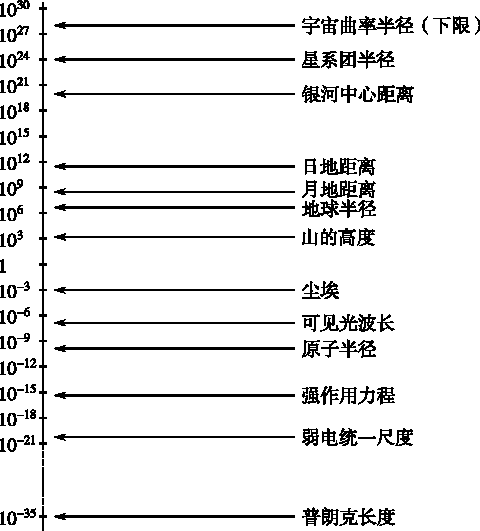
\includegraphics{figure/tab01.03.pdf} \\
        \bottomrule
    \end{tabular}
\end{tablex}
\clearpage

\noindent 了新的米的定义,即用光速值来定义“米”,以代替1960年的规定。
新的米的定义是,米是光在真空中在1,299,792,458秒的时间间隔
内所传播的路程长度。按这种新的定义,光速c是一固定的常数,即

\centerline{$c$=299,792,458米/秒}

表\ref{tab:01.03}~中列举了一些典型现象的空间尺度。目前,物理学中涉
及的最太长度是$10^{28}$米,它是宇宙曲率半径的下限;已达到的最
小长度为$10^{-20}$米,它是弱电统一的特征尺度。普朗克长度约为
$10^{-35}$米,被认为是最小的长度,意思是说,在比普朗克长度更小
的范围内,长度的概念可能就不再适用了。
